\subsection{Section 7.3}

\begin{tcolorbox}[
        title={Problem 16},
        valign=center,
        nobeforeafter,
        colframe=gray!95!black
    ]
    Find a parametrization of the surface
    \begin{align}
        x^3 + 3xy + z^2 &= 2
    \end{align}
    where \(z \geq 0\). \\
    
    Use it to find the tangent plane at the point \((x, y, z) = \left(1, \frac{1}{3}, 0\right)\).
\end{tcolorbox}

\begin{solution}
    Recall that we parametrize a surface using the function \(\Phi: D \subset \mathbb{R}^2 \rightarrow S \subset \mathbb{R}^3\):
    \begin{align}
        \Phi(u, v) &= (x, y, z)
    \end{align}
    
    Observe that it is easier to isolate for \(y\) in terms of \(x\) and \(z\). This is because there is a cubed term in \(x\) and a squared term in \(z\).
    
    We therefore parametrize this surface by first setting \(x = u\) and \(z = v\).
    
    Isolating for \(y\):
    \begin{align*}
        2 &= x^3 + 3xy + z^2 \\
        -3xy &= x^3 + z^2 - 2 \\
        y &= -\frac{x^3 + z^2 - 2}{3x} \\
        y &= -\frac{x^2}{3} - \frac{z^2}{3x} + \frac{2}{3x} \\
        y &= -\frac{u^2}{3} - \frac{v^2}{3u} + \frac{2}{3u}
    \end{align*}
    
    Then:
    \begin{align}
        \Phi(u, v) &= \left(u, -\frac{u^2}{3} - \frac{v^2}{3u} + \frac{2}{3u}, v\right)
    \end{align}
    
    In order to find the tangent plane at a given point, we must first compute the normal vector of the surface at that point.
    
    Recall that the normal vector of the parametrized surface is given by:
    \begin{align}
        \vec{n} &= \Phi_u \times \Phi_v
    \end{align}
    
    We now compute the partial derivatives of \(\Phi\):
    \begin{align}
        \Phi_u &= \left(1, -\frac{2u}{3} + \frac{v^2}{3u^2} - \frac{2}{3u^2}, 0\right) & \Phi_v &= \left(0, - \frac{2v}{3u}, 1\right)
    \end{align}
    
    Observe that the point \((x, y, z) = \left(1, \frac{1}{3}, 0\right)\) is given by \((u, v) = (1, 0)\).
    
    Then the normal at the point \((x, y, z) = \left(1, \frac{1}{3}, 0\right)\) is given by:
    \begin{align*}
        \vec{n} &= \Phi_u(1, 0) \times \Phi_v(1, 0) \\
        &= \left(1, -\frac{2(1)}{3} + \frac{(0)^2}{3(1)^2} - \frac{2}{3(1)^2}, 0\right) \times \left(0, - \frac{2(0)}{3(1)}, 1\right) \\
        &= \left(1, -\frac{2}{3} - \frac{2}{3}, 0\right) \times \left(0, 0, 1\right) \\
        &= \left(1, -\frac{4}{3}, 0\right) \times \left(0, 0, 1\right) \\
        &= \left(1, -\frac{4}{3}, 0\right) \times \left(0, 0, 1\right) \\
        &= \left(-\frac{4}{3}, -1, 0\right)
    \end{align*}
    
    Recall that the equation of the plane tangent to the point \((x_0, y_0, z_0)\) is given by:
    \begin{align}
        \vec{n} \cdot \left((x, y, z) - (x_0, y_0, z_0)\right) &= 0 \\
        \vec{n} \cdot \left(x - x_0, y - y_0, z - z_0\right) &= 0
    \end{align}
    
    Then the equation of the plane tangent to the point \(\left(1, \frac{1}{3}, 0\right)\) is given by:
    \begin{align*}
        \vec{n} \cdot \left(x - x_0, y - y_0, z - z_0\right) &= 0 \\
        \left(-\frac{4}{3}, -1, 0\right) \cdot \left(x - 1, y - \frac{1}{3}, z\right) &= 0 \\
        -\frac{4}{3}(x - 1) - \left(y - \frac{1}{3}\right) &= 0 \\
        -\frac{4}{3}x + \frac{4}{3} - y + \frac{1}{3} &= 0 \\
        \frac{4}{3}x + y - \frac{5}{3} &= 0
    \end{align*}
    
\end{solution}

\begin{tcolorbox}[
        title={Problem 18},
        valign=center,
        nobeforeafter,
        colframe=gray!95!black
    ]
    Given a sphere of radius 2 centered at the origin, find the equation for the plane tangent to it at the point \((1, 1, \sqrt{2})\) by considering the sphere as:
    
    \begin{itemize}
        \item a sphere parametrized by \(\Phi(\theta, \phi) = (2\cos(\theta)\sin(\phi), 2\sin(\theta)\sin(\phi), 2\cos(\phi))\)
        \item a level surface of \(f(x, y, z) = x^2 + y^2 + z^2\)
        \item the graph of \(g(x, y) = \sqrt{4 - x^2 - y^2}\)
    \end{itemize}
\end{tcolorbox}

\begin{solution}
\textit{(Parametrization)}

Recall that for an arbitrary parametrization \(\Phi(u, v)\), the vector \(\Phi_u \times \Phi_v\) is the normal vector to the parametrized surface \(S\).

Then the vector \(\Phi_\theta \times \Phi_\phi\) is the normal vector of the sphere.

We compute the partial derivatives of \(\Phi\):
\begin{align*}
    \Phi_\theta &= (-2\sin(\theta)\sin(\phi), 2\cos(\theta)\sin(\phi), 0) & \Phi_\phi &= (2\cos(\theta)\cos(\phi), 2\sin(\theta)\cos(\phi), -2\sin(\phi))
\end{align*}

Observe that the point \((1, 1 \sqrt{2})\) is given by \((\theta, \phi) = \left(\frac{\pi}{4}, \frac{\pi}{4}\right)\). 

This can be found by equating the point of interest with the parametrization and solving for \(\theta\) and \(\phi\) component-wise:
\begin{align*}
    (1, 1 \sqrt{2}) &= (2\cos(\theta)\sin(\phi), 2\sin(\theta)\sin(\phi), 2\cos(\phi))
\end{align*}

We first solve for \(\phi\) by analyzing the \(z\) component:
\begin{align*}
    2\cos{\phi} &= \sqrt{2} \\
    \cos{\phi} &= \frac{\sqrt{2}}{2} \\
    \phi &= \pm \frac{\pi}{4}
\end{align*}

By convention, \(\phi \in [0, \pi]\). Therefore, \(\phi = \frac{\pi}{4}\).

We now solve for \(\theta\) by analyzing the \(x\) and \(y\) components:
\begin{align*}
    2\cos(\theta)\sin(\phi) &= 1 & 2\sin(\theta)\sin(\phi) &= 1 \\
    2\cos(\theta)\sin\left(\frac{\pi}{4}\right) &= 1 & 2\sin(\theta)\sin\left(\frac{\pi}{4}\right) &= 1 \\
    2\cos(\theta)\frac{\sqrt{2}}{2} &= 1 & 2\sin(\theta)\frac{\sqrt{2}}{2} &= 1 \\
    \sqrt{2} \cos(\theta) &= 1 & \sqrt{2} \sin(\theta) &= 1 \\
    \cos(\theta) &= \frac{1}{\sqrt{2}} & \sin(\theta) &= \frac{1}{\sqrt{2}} \\
    \theta &= \pm \frac{\pi}{4} & \theta &= \frac{\pi}{4} \text{ or } \frac{3\pi}{4}
\end{align*}

Both conditions hold when \(\theta = \frac{\pi}{4}\).

Then the normal at the point \((1, 1 \sqrt{2})\) is given by:
\begin{align*}
    \vec{n} &= \Phi_\theta\left(\frac{\pi}{4}, \frac{\pi}{4}\right) \times \Phi\left(\frac{\pi}{4}, \frac{\pi}{4}\right) \\
    &= \left(-2\sin\left(\frac{\pi}{4}\right)\sin\left(\frac{\pi}{4}\right), 2\cos\left(\frac{\pi}{4}\right)\sin\left(\frac{\pi}{4}\right), 0\right) \times \left(2\cos\left(\frac{\pi}{4}\right)\cos\left(\frac{\pi}{4}\right), 2\sin\left(\frac{\pi}{4}\right)\cos\left(\frac{\pi}{4}\right), -2\sin\left(\frac{\pi}{4}\right)\right) \\
    &= \left(-2\frac{\sqrt{2}}{2}\frac{\sqrt{2}}{2}, 2\frac{\sqrt{2}}{2}\frac{\sqrt{2}}{2}, 0\right) \times \left(2\frac{\sqrt{2}}{2}\frac{\sqrt{2}}{2}, 2\frac{\sqrt{2}}{2}\frac{\sqrt{2}}{2}, -2\frac{\sqrt{2}}{2}\right) \\
    &= \left(-\frac{2}{2}, \frac{2}{2}, 0\right) \times \left(\frac{2}{2}, \frac{2}{2}, -\sqrt{2}\right) \\
    &= \left(-1, 1, 0\right) \times \left(1, 1, -\sqrt{2}\right) \\
    &= \left(\sqrt{2}, \sqrt{2}, 2\right)
\end{align*}

Recall that the equation of the plane tangent to the point \((x_0, y_0, z_0)\) is given by:
    \begin{align}
        \vec{n} \cdot \left((x, y, z) - (x_0, y_0, z_0)\right) &= 0 \\
        \vec{n} \cdot \left(x - x_0, y - y_0, z - z_0\right) &= 0
    \end{align}
    
    Then the equation of the plane tangent to the point \(\left(1, 1, \sqrt{2}\right)\) is given by:
    \begin{align*}
        \vec{n} \cdot \left(x - x_0, y - y_0, z - z_0\right) &= 0 \\
        \left(\sqrt{2}, \sqrt{2}, 2\right) \cdot \left(x - 1, y - 1, z - \sqrt{2}\right) &= 0 \\
        \sqrt{2}(x - 1) + \sqrt{2}(y - 1) + 2\left(z - \sqrt{2}\right) &= 0 \\
        \sqrt{2}x - \sqrt{2} + \sqrt{2}y - \sqrt{2} + 2z - 2\sqrt{2} &= 0 \\
        \sqrt{2}x + \sqrt{2}y + 2z - 4\sqrt{2} &= 0 \\
        x + y + \sqrt{2}z - 4 &= 0
    \end{align*}

\end{solution}

\begin{solution}
\textit{(Level surface)}
    
    Observe that the sphere of radius 2 centered at the origin is equal to the level surface of \(f\) where \(f(x, y, z) = 4\).
    
    Recall that the gradient of \(f\) is perpendicular to every level surface of \(f\). The normal vector is therefore parallel to the gradient of \(f\).
    
    We first compute the gradient of \(f\):
    \begin{align}
        \nabla f &= (2x, 2y, 2z)
    \end{align}
    
    Then the normal at the point \((x, y, z) = (1, 1, \sqrt{2})\) is given by:
    \begin{align*}
        \vec{n} &= \nabla f(1, 1, \sqrt{2}) \\
        &= (2(1), 2(1), 2\sqrt{2}) \\
        &= (2, 2, 2\sqrt{2})
    \end{align*}
    
    Recall that the equation of the plane tangent to the point \((x_0, y_0, z_0)\) is given by:
    \begin{align}
        \vec{n} \cdot \left((x, y, z) - (x_0, y_0, z_0)\right) &= 0 \\
        \vec{n} \cdot \left(x - x_0, y - y_0, z - z_0\right) &= 0
    \end{align}
    
    Then the equation of the plane tangent to the point \(\left(1, 1, \sqrt{2}\right)\) is given by:
    \begin{align*}
        \vec{n} \cdot \left(x - x_0, y - y_0, z - z_0\right) &= 0 \\
        (2, 2, 2\sqrt{2}) \cdot \left(x - 1, y - 1, z - \sqrt{2}\right) &= 0 \\
        2(x - 1) + 2(y - 1) + 2\sqrt{2}(z - \sqrt{2}) &= 0 \\
        2x - 2 + 2y - 2 + 2\sqrt{2}z - 4 &= 0 \\
        2x + 2y + 2\sqrt{2}z - 8 &= 0 \\
        x + y + \sqrt{2}z - 4 &= 0
    \end{align*}
    
\end{solution}

\begin{solution}
\textit{(Graph)}
    
    Recall that the equation of the plane tangent to the graph of \(g\) at \((x_0, y_0, g(x_0, y_0))\) is given by:
    \begin{align}
        z - g(x_0, y_0) &= \frac{\partial g(x_0, y_0)}{\partial x}(x - x_0) + \frac{\partial g(x_0, y_0)}{\partial y}(y - y_0)
    \end{align}
    
    We first calculate the partial derivatives of \(g\):
    \begin{align*}
        \frac{\partial g}{\partial x} &= -\frac{x}{\sqrt{4 - x^2 - y^2}} & \frac{\partial g}{\partial y} &= -\frac{y}{\sqrt{4 - x^2 - y^2}}
    \end{align*}
    
    The equation of the plane tangent to the graph of \(g\) at \((1, 1, \sqrt{2})\) is then given by:
    \begin{align*}
        z - \sqrt{2} &= -\frac{1}{\sqrt{4 - 1^2 - 1^2}}(x - 1) -\frac{1}{\sqrt{4 - 1^2 - 1^2}}(y - 1) \\
        z - \sqrt{2} &= -\frac{1}{\sqrt{4 - 2}}(x - 1) -\frac{1}{\sqrt{4 - 2}}(y - 1) \\
        z - \sqrt{2} &= -\frac{1}{\sqrt{2}}(x - 1) -\frac{1}{\sqrt{2}}(y - 1) \\
        \sqrt{2} z - 2 &= -(x - 1) -(y - 1) \\
        0 &= x - 1 + y - 1 + \sqrt{2} z - 2 \\
        0 &= x + y + \sqrt{2} z - 4
    \end{align*}
\end{solution}

\subsection{Section 7.4}

\begin{tcolorbox}[
        title={Problem 6},
        valign=center,
        nobeforeafter,
        colframe=gray!95!black
    ]
    Find the area of the surface defined by \(z = xy\) and \(x^2 + y^2 \leq 2\).
\end{tcolorbox}

\begin{solution}
    Observe that this surface is given in the form \(z = g(x, y)\). 
    
    Recall that the area of a graph is given by:
    \begin{align}
        A(S) &= \iint_D \sqrt{1 + \|\nabla g\|^2} \ dA
    \end{align}
    
    We first calculate the gradient:
    \begin{align}
        \nabla g &= \left(\frac{\partial g}{\partial x}, \frac{\partial g}{\partial y}\right) \\
        &= \left(y, x\right)
    \end{align}
    
    We now calculate the norm of the gradient:
    \begin{align}
        \|\nabla g\|^2 &= \|\left(y, x\right)\|^2 \\
        &= y^2 + x^2
    \end{align}
    
    The integral is easier to compute in polar coordinates. Therefore, we will compute the integral in polar coordinates.
    
    Recall that:
    \begin{align}
        x &= r\cos(\theta) & y &= r\sin(\theta) & r &= \sqrt{x^2 + y^2}
    \end{align}
    
    Then the domain of integration is given by:
    \begin{align}
        0 \leq & \ r \leq \sqrt{2} & 0 \leq & \ \theta \leq 2\pi
    \end{align}
    
    Recall also that the infinitesimal area element in polar coordinates is given by:
    \begin{align}
        dA &= r \ dr d\theta
    \end{align}
    
    Then the surface area is given by:
    \begin{align}
        A(S) &= \iint_D \sqrt{1 + \|\nabla g\|^2} \ dA \\
        &= \iint_D \sqrt{1 + y^2 + x^2} \ dA \\
        &= \int_0^{2\pi} \int_0^{\sqrt{2}} \sqrt{1 + r^2} \ r \ dr d\theta \\
        &= \int_0^{2\pi} \frac{1}{3}\left(\sqrt{1 + r^2}\right)^{\frac{3}{2}}\Biggr|_0^{\sqrt{2}} d\theta \\
        &= \frac{1}{3}\int_0^{2\pi} \sqrt{1 + \sqrt{2}^2} - \sqrt{1 + 0^2} \ d\theta \\
        &= \frac{1}{3} \int_0^{2\pi} \sqrt{3} - 1 \ d\theta \\
        &= \frac{2\pi}{3} \left(\sqrt{3} - 1\right)
    \end{align}
\end{solution}

\begin{tcolorbox}[
        title={Problem 10},
        valign=center,
        nobeforeafter,
        colframe=gray!95!black
    ]
    Find the area of the portion of the unit sphere that is cut out by the cone \(z \geq \sqrt{x^2 + y^2}\).
\end{tcolorbox}

\begin{solution}
    The intersection of the sphere and the cone is found by equation the following two equations:
    \begin{align*}
        x^2 + y^2 + z^2 &= 1 & z &= \sqrt{x^2 + y^2}
    \end{align*}
    
    We obtain:
    \begin{align*}
        x^2 + y^2 + z^2 &= 1 \\
        x^2 + y^2 + \left(\sqrt{x^2 + y^2}\right)^2 &= 1 \\
        x^2 + y^2 + x^2 + y^2 &= 1 \\
        2x^2 + 2y^2 &= 1 \\
        x^2 + y^2 &= \frac{1}{2} \\
        \sqrt{x^2 + y^2} &= \frac{1}{\sqrt{2}}
    \end{align*}
    
    It follows that \(z = \frac{1}{\sqrt{2}}\). 
    
    \begin{figure}[h!]
        \centering
        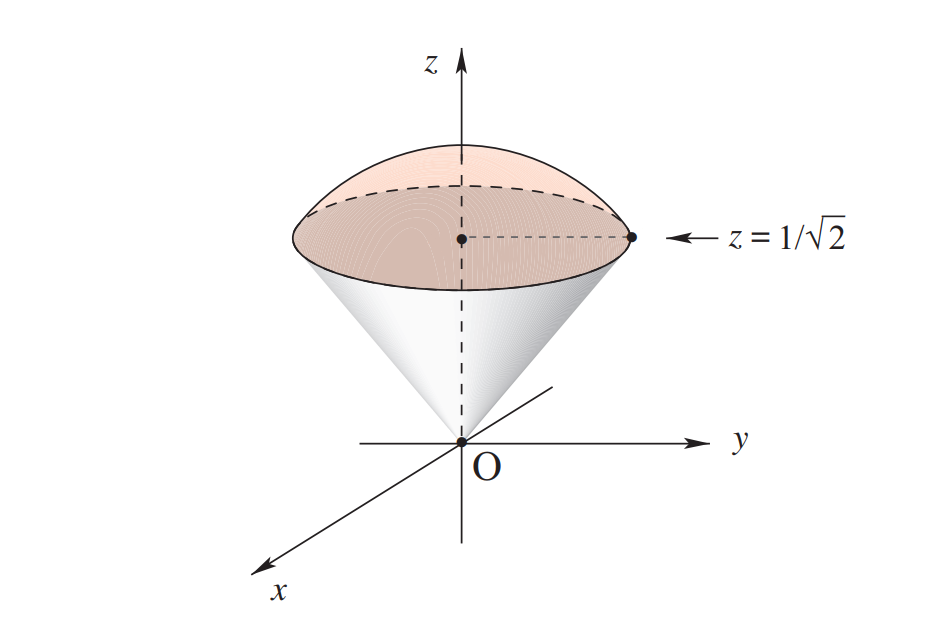
\includegraphics[width=0.4\textwidth]{Pictures/Tutorial 7-1.png}
        \caption{Area of the portion of the unit sphere enclosed by the cone \(z \geq \sqrt{x^2 + y^2}\).}
    \end{figure}
    
    Recall that the parametrization of the surface area of the unit sphere is given by:
    \begin{align}
        \Phi(\theta, \phi) &= (x, y, z) \\
        &= (\cos(\theta)\sin(\phi), \sin(\theta)\sin(\phi), \cos(\phi))
    \end{align}
    where \(0 \leq \theta \leq 2\pi\) and \(0 \leq \phi \leq \pi\).
    
    Since we want to find the surface area of the sphere enclosed by the cone, we must first find the bounds of our integral in terms of \(\theta\) and \(\phi\).
    
    From the figure, observe that \(0 \leq \theta < 2\pi\). The bounds for the angle \(\theta\) remain unchanged.
    
    However, observe also that:
    \begin{align*}
        \frac{1}{\sqrt{2}} \leq & \ z \leq 1 \\
        \frac{1}{\sqrt{2}} \leq & \ \cos(\phi) \leq 1
    \end{align*}
    
    We find that \(0 \leq \phi \leq \frac{\pi}{4}\).
    
    Recall that the area of a parametrized surface is given by:
    \begin{align}
        A(S) &= \iint_D \|\Phi_u \times \Phi_v \| \ dudv
    \end{align}
    
    We know from spherical coordinates that the norm of the cross product is equal to the Jacobian:
    \begin{align}
        \|\Phi_\theta \times \Phi_\phi \| &= \left|\frac{\partial(x, y, z)}{\partial(\rho, \theta, \phi)}\right| \\
        &= \rho^2\sin(\phi)
    \end{align}
    
    Since \(\rho = 1\), we have that:
    \begin{align*}
        \|\Phi_\theta \times \Phi_\phi \| &= \sin(\phi)
    \end{align*}
    
    Then the surface area of the sphere enclosed by the cone is given by:
    \begin{align*}
        A(S) &= \iint_D \|\Phi_\theta \times \Phi_\phi \| \ d\theta d\phi \\
        &= \int_0^{\frac{\pi}{4}} \int_0^{2\pi} \sin(\phi) \ d\theta d\phi \\
        &= 2\pi \int_0^{\frac{\pi}{4}} \sin(\phi) \ d\phi \\
        &= -2\pi \cos(\phi) \Big|_0^{\frac{\pi}{4}} \\
        &= -2\pi \cos\left(\frac{\pi}{4}\right) + 2\pi \cos(0)  \\
        &= -\frac{2\pi}{\sqrt{2}} + 2\pi \\
        &= 2\pi\left(1 -\frac{1}{\sqrt{2}}\right)
    \end{align*}
\end{solution}